\documentclass[12pt,letterpaper]{article}

%% === margins / layout ===
\usepackage[margin=1in]{geometry}
\usepackage{iftex}
\ifPDFTeX
  \pdfminorversion=4
\fi

%% === basic packages ===
\ifPDFTeX
  \usepackage[T1]{fontenc}
  \usepackage[utf8]{inputenc}
  \usepackage{lmodern}
\else
  \usepackage{fontspec}
  \setmainfont{Times New Roman}
  \setsansfont{Helvetica}
  \setmonofont{Menlo}
  % Render non-Latin scripts in trace tables without manual font switching.
  \ifXeTeX
    \usepackage{ucharclasses}
    \newfontfamily\armenianfont{Mshtakan}
    \setTransitionsFor{Armenian}{\armenianfont}{\normalfont}
  \fi
\fi
\usepackage{microtype}
\usepackage{latexsym}
\usepackage{amssymb,amsmath,bm}
\usepackage{mathtools}
\usepackage{booktabs}
\usepackage{graphicx}
\usepackage{float}
\usepackage{enumitem}
\usepackage{setspace}
\usepackage{placeins}
\newcommand\spacingset[1]{\setstretch{#1}}

%% === tables for trace examples ===
\usepackage{ragged2e}
\usepackage{tabularx}
\usepackage[table]{xcolor}
\usepackage{threeparttable}
\definecolor{RowShade}{gray}{0.96}
\newcolumntype{P}[1]{>{\RaggedRight\arraybackslash}p{#1}}
\newcolumntype{C}[1]{>{\Centering\arraybackslash}p{#1}}
\newcolumntype{Y}{>{\RaggedRight\arraybackslash}X}

%% === hyperlinks ===
\usepackage[bookmarksopen=true, bookmarksnumbered=true,
pdfstartview=FitH, breaklinks=true,
urlbordercolor={0 1 0}, citebordercolor={0 0 1}]{hyperref}

%% === TikZ ===
\usepackage{tikz}
\usetikzlibrary{arrows.meta,calc,positioning,fit,shapes.geometric,shapes.misc,backgrounds}

%% === bibliography ===
\usepackage[natbib=true,minnames=1,maxnames=3,backend=biber,style=authoryear-luh-ipw]{biblatex}
\addbibresource{mybib.bib}

%% === figure path ===
\graphicspath{{./../Figures/}}

%% === stats macros (generated) ===
\newcommand{\LLMOverallAccAllpolparty}{0.751}
\newcommand{\LLMOverallAccHighpolparty}{0.860}
\newcommand{\LLMMeanLowConfpolparty}{0.250}
\newcommand{\LLMMedianLowConfpolparty}{0.250}
\newcommand{\LLMMeanAccByCountryHighpolparty}{0.879}
\newcommand{\LLMMeanBaselineByCountrypolparty}{0.536}
\newcommand{\LLMMeanDeltaByCountrypolparty}{0.343}
\newcommand{\LLMMinDeltaByCountrypolparty}{-0.602}
\newcommand{\LLMMaxDeltaByCountrypolparty}{0.761}
\newcommand{\LLMMinDeltaCountrypolparty}{Gambia}
\newcommand{\LLMMaxDeltaCountrypolparty}{Finland}
\newcommand{\LLMMeanAccSmallGroupspolparty}{0.692}
\newcommand{\LLMMeanAccLargeGroupspolparty}{0.820}
\newcommand{\LLMNumCountriespolparty}{114}
\newcommand{\LLMNumInstancespolparty}{34,618}
\newcommand{\LLMNumClassespolparty}{1,209}
\newcommand{\LLMNumPredictionsGainedpolparty}{12,898}
\newcommand{\LLMNumPredictionsGainedPercentpolparty}{20.8}
\newcommand{\LLMRelaxedChangedPctpolparty}{2.5}


\title{A Verifiable Search Agent Methodology at Scale for Political Elite Research}
\author{Final author list TBD}
\date{}

\begin{document}
\maketitle
\spacingset{1.25}

\begin{abstract}
\noindent Large-\(N\) political-elite datasets increasingly rely on digital traces, but scaling elite attribute coding with ``search-enabled LLMs'' raises three methodological hazards for inference and replication: (i) \emph{non-verifiability} (answers without durable evidence trails), (ii) \emph{non-comparability} (open-ended labels that drift across countries and time), and (iii) \emph{temporal leakage} (using post-period information to code pre-period attributes, a close analogue of post-treatment conditioning in causal inference).
We present a \emph{verifiable search agent} methodology that treats web retrieval as a measurement instrument whose inputs, outputs, and timing are explicitly governed and archived.
The agent executes short, provenance-preserving search sessions; constrains decisions to expert-supplied closed codebooks; produces structured, citation-backed outputs; abstains under weak or conflicting evidence; and stores complete traces for audit and re-analysis.
In a party-affiliation labeling task spanning \LLMNumCountriespolparty{} countries (\(N=\) \LLMNumInstancespolparty{} matched leader--records; \LLMNumClassespolparty{} party labels), the high-confidence accuracy is \LLMOverallAccHighpolparty{} while expanding usable coverage by \LLMNumPredictionsGainedPercentpolparty{}\% (\LLMNumPredictionsGainedpolparty{} previously missing labels) with a conservative abstention layer.
\end{abstract}
\vspace{0.4em}
\noindent\textbf{Keywords:} political elites; measurement; tool-using retrieval; replication; temporal leakage.

\begin{figure}[htb]
  \centering
  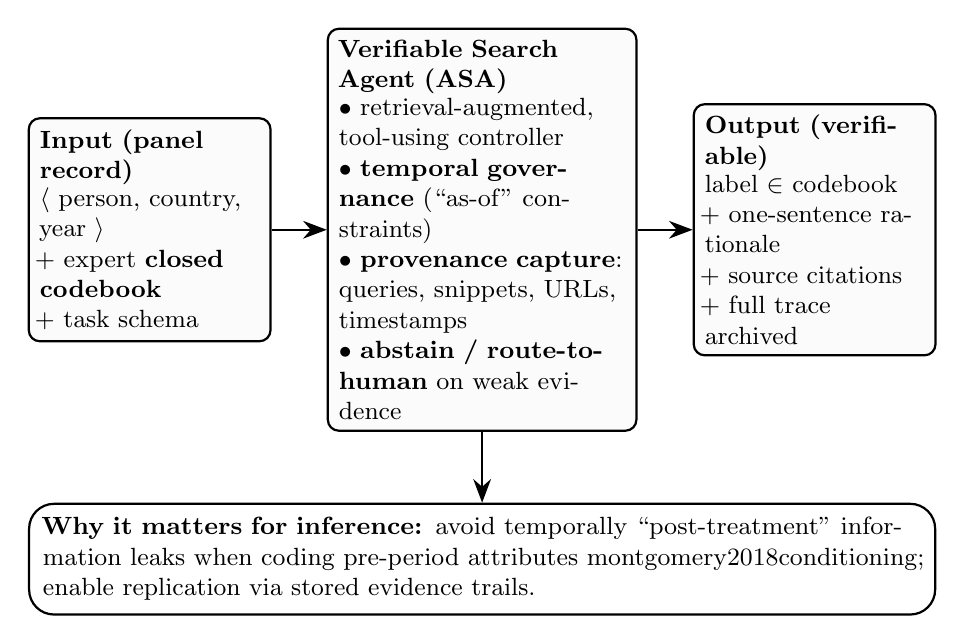
\begin{tikzpicture}[
    font=\small,
    node distance=9mm and 7mm,
    box/.style={rounded corners, draw=black, thick, fill=gray!3, inner sep=4pt, align=left},
    pill/.style={rounded corners=9pt, draw=black, thick, fill=white, inner sep=5pt, align=left},
    arr/.style={-{Stealth[length=3mm]}, thick},
  ]
    \node[box, text width=0.23\linewidth] (input) {
      \textbf{Input (panel record)}\\[-1pt]
      \(\langle\) person, country, year \(\rangle\)\\
      + expert \textbf{closed codebook}\\
      + task schema
    };

    \node[box, right=of input, text width=0.30\linewidth] (agent) {
      \textbf{Verifiable Search Agent (ASA)}\\[-1pt]
      \(\bullet\) retrieval-augmented, tool-using controller\\
      \(\bullet\) \textbf{temporal governance} (``as-of'' constraints)\\
      \(\bullet\) \textbf{provenance capture}: queries, snippets, URLs, timestamps\\
      \(\bullet\) \textbf{abstain / route-to-human} on weak evidence
    };

    \node[box, right=of agent, text width=0.23\linewidth] (output) {
      \textbf{Output (verifiable)}\\[-1pt]
      label \(\in\) codebook\\
      + one-sentence rationale\\
      + source citations\\
      + full trace archived
    };

    \draw[arr] (input) -- (agent);
    \draw[arr] (agent) -- (output);

    \node[pill, below=9mm of agent, text width=0.92\linewidth] (why) {
      \textbf{Why it matters for inference:} avoid temporally ``post-treatment'' information leaks when coding pre-period attributes \citep{montgomery2018conditioning}; enable replication via stored evidence trails.
    };
    \draw[arr] (agent.south) -- (why.north);
  \end{tikzpicture}%
  \caption{Visual abstract: the ASA treats web retrieval as a governed, auditable measurement process rather than an opaque chat interaction.}
  \label{fig:visual-abstract}
\end{figure}

\section{Introduction}

Large-\(N\) political-elite datasets underpin research on representation, accountability, and governance, but assembling them requires repeated, error-prone measurement of categorical attributes (e.g., party affiliation) across countries and time.
As digital traces proliferate, it is tempting to scale attribute coding by asking search-enabled large language models (LLMs) for answers.
Yet, interactive question answering is not a measurement protocol: without explicit governance, such workflows tend to be difficult to audit, hard to replicate, and vulnerable to temporally invalid evidence.

We argue that retrieval-augmented LLM agents can be useful for dataset construction only when they are treated as \emph{governed instruments}.
We present a \emph{verifiable search agent} methodology, implemented in the \texttt{asa} software stack, that formalizes retrieval as measurement: for each record \(\langle\)person, country, year\(\rangle\) and an expert-supplied closed codebook, the agent runs a short, budgeted search session; prioritizes evidence over parametric recall; emits a structured output with citations; abstains under weak or conflicting evidence; and archives a complete trace (queries, snippets, URLs, timestamps) for later audit and re-analysis.

\paragraph{Contributions.}
First, we identify three hazards that make ``search-enabled coding'' non-standard as a research workflow: (i) non-verifiability, (ii) non-comparability, and (iii) temporal leakage (a close analogue of post-treatment conditioning in causal inference).
Second, we translate these hazards into a concrete protocol with closed-world decisions, evidence-first outputs, temporal governance, and conservative abstention.
Third, we validate the methodology on party-affiliation labeling, a verifiable elite attribute with an expert closed codebook.

\paragraph{Preview of results.}
In the party-affiliation task spanning \LLMNumCountriespolparty{} countries (\(N=\) \LLMNumInstancespolparty{} matched leader--records; \LLMNumClassespolparty{} party labels), ASA achieves high-confidence accuracy \LLMOverallAccHighpolparty{} while expanding usable coverage by \LLMNumPredictionsGainedPercentpolparty{}\% (\LLMNumPredictionsGainedpolparty{} previously missing labels) and withholding \LLMMeanLowConfpolparty{} of cases on average via an abstention gate.
Relative to a simple country-majority baseline (\LLMMeanBaselineByCountrypolparty{}), the mean uplift in high-confidence accuracy is \LLMMeanDeltaByCountrypolparty{}.

\paragraph{Roadmap.}
Section~\ref{sec:hazards} motivates the design by formalizing three measurement hazards.
Section~\ref{sec:related} situates the contribution in political methodology, reproducible research, and recent retrieval-agent architectures.
Sections~\ref{sec:method}--\ref{sec:validation} describe the ASA protocol and validate it on party affiliation.
We conclude with guidance on transparency, limitations, and ethical considerations for web-based measurement.

\section{Measurement hazards in search-enabled coding\label{sec:hazards}}

Digital sources make it feasible to code political-elite attributes at scale, but research-grade datasets impose requirements that differ from interactive question answering.
In practice, a default workflow---``ask a search-enabled model for the answer''---tends to fail on three dimensions central to quantitative political science.

\paragraph{Auditability and replication.}
Elite attribute labels are \emph{measurements}. When the underlying retrieval context is not archived (queries, results, snippets, URLs, timestamps), a label is difficult to verify and cannot be re-audited when coders disagree or sources change.
This is especially problematic for downstream users who need to understand measurement error and may wish to apply alternative inclusion rules (e.g., discarding any label lacking a primary source).

\paragraph{Cross-national comparability.}
Many elite variables are \emph{categorical} and country-specific (e.g., party labels). ``Open-world'' generation invites label drift (synonyms, translations, rebrandings), undermining comparability across countries and years.
Closed codebooks supplied by domain experts are a natural remedy, but generic search-enabled chat systems do not typically enforce them.

\paragraph{Temporal leakage and post-treatment bias.}
Political elites switch parties, offices, and coalitions. If coding for year \(t\) uses sources written after \(t\) (e.g., biographies updated in 2025), the measurement can incorporate information that is itself caused by post-\(t\) outcomes.
This is a close analogue of conditioning on post-treatment variables in causal inference \citep{montgomery2018conditioning}: a label intended to reflect the pre-period state may be contaminated by later events, inducing bias in estimated relationships.
Temporal governance therefore belongs \emph{inside} the measurement protocol, not in ad hoc post-hoc cleaning.

\paragraph{Design implications.}
These hazards motivate treating retrieval as a governed measurement instrument: decisions must be constrained (closed codebooks), evidence must be preserved (citations and traces), time must be part of the protocol (``as-of'' rules), and weak evidence should trigger abstention rather than guessing.
Table~\ref{tab:hazard-mitigation} summarizes how ASA operationalizes these requirements.

\begin{table}[htb]
\centering
\caption{Common hazards in search-enabled coding and ASA design responses.}
\label{tab:hazard-mitigation}
\small
\begin{tabularx}{\linewidth}{@{}>{\RaggedRight\arraybackslash}p{0.30\linewidth}X@{}}
\toprule
\textbf{Hazard} & \textbf{ASA response} \\
\midrule
Non-verifiability (answers without durable evidence trails) &
Evidence-first outputs with explicit citations; full trace capture (queries, snippets, URLs, timestamps) for audit and re-analysis. \\
Non-comparability (label drift across countries/time) &
Closed-world decisions constrained to expert codebooks, plus conservative post-processing that normalizes benign surface variation without introducing new classes. \\
Temporal leakage (post-period information used for pre-period labels) &
Explicit ``as-of'' rules with date verification where feasible; warnings and abstention rather than silently relying on potentially post-period sources. \\
\bottomrule
\end{tabularx}
\end{table}

\section{Related work\label{sec:related}}

Our contribution sits at the intersection of political methodology and recent advances in retrieval-augmented language models.
Large cross-national datasets often rely on expert coding and bespoke compilation efforts; a central challenge is preserving comparability and documenting measurement decisions at scale.
ASA complements such efforts by treating web retrieval as a first-class part of the measurement protocol and by archiving evidence trails that allow downstream users to audit labels and re-apply inclusion rules.
The validation task we study is motivated by the same large-\(N\) political-elite measurement agenda that underlies recent work on global leadership and expert-coded cross-national datasets \citep{gerring2019rules,pemstein2020v}.

ASA is also aligned with calls for reproducible computational research: replication requires not only code, but durable documentation of the information environment that produced a label \citep{peng2011reproducible,stodden2013toward}.
In web-based measurement, the information environment is inherently dynamic; capturing queries, snippets, URLs, and timestamps makes it possible to re-audit outputs when sources change.
Our emphasis on temporal governance connects directly to concerns about look-ahead and leakage when post-period information is used to measure pre-period covariates \citep{kaufman2012leakage,montgomery2018conditioning}.

On the NLP side, retrieval-augmented generation and tool-using agents provide building blocks for ASA's implementation \citep{lewis2020retrieval,yao2022react}.
However, the core contribution here is not a new prompting trick or a larger model; it is a measurement-oriented design that prioritizes comparability, auditability, and temporal validity over unconstrained answer generation.

\section{Methodology: a verifiable search agent\label{sec:method}}

We present a protocol---implemented as the \texttt{asa} software stack---that makes agent-based retrieval \emph{verifiable by construction}.
The methodology separates (i) a task-level specification that defines what constitutes admissible evidence and outputs, from (ii) an implementation that executes the specification and persists traces.

\subsection{Protocol commitments}

The protocol has four core commitments:
\begin{enumerate}[leftmargin=*, itemsep=2pt]
\item \textbf{Closed-world decisions.} All predictions must lie in an expert-supplied codebook (e.g., the parties observed in a country-year panel).
\item \textbf{Evidence-first outputs.} Each label is paired with a terse rationale anchored to explicit source citations.
\item \textbf{Provenance preservation.} The system archives the full interaction trace: queries, tool responses, extracted snippets, URLs, and timestamps.
\item \textbf{Conservative abstention.} Under weak or conflicting evidence, the agent abstains (or routes to humans) rather than guessing.
\end{enumerate}

\subsection{Task formalization}

For each target record \(i\), the inputs are: a person name, a target country, an observation year \(t_i\), and a closed codebook \(\mathcal{C}_i\) supplied by expert coders.
The agent must return either (a) a label \(c \in \mathcal{C}_i\) with citations, or (b) an abstention.

\subsection{Implementation: ASA software stack}

Operationally, the agent runs a short search session with read-only retrieval tools (e.g., Wikipedia and general web search), compiles candidate evidence, and emits a structured JSON result (label, one-sentence justification with citations, and a confidence category).
This design follows retrieval-augmented, tool-using agent patterns in the recent NLP literature \citep{yao2022react,lewis2020retrieval}.
The implementation is designed to be \emph{task-configurable}: domain experts supply the closed codebook and task schema, while the shared execution layer enforces the protocol commitments (trace capture, abstention, and evidence-first outputs).

A conservative post-processor then normalizes the label against the codebook: exact-match acceptance first, followed by a guarded fuzzy match for benign surface variation (punctuation, plurals, acronyms) using high similarity thresholds.
This reduces typographic drift without introducing new classes; in the party-affiliation case study, the relaxed mapper changes \LLMRelaxedChangedPctpolparty{}\% of accepted labels.

\begin{figure}[htb]
  \centering
  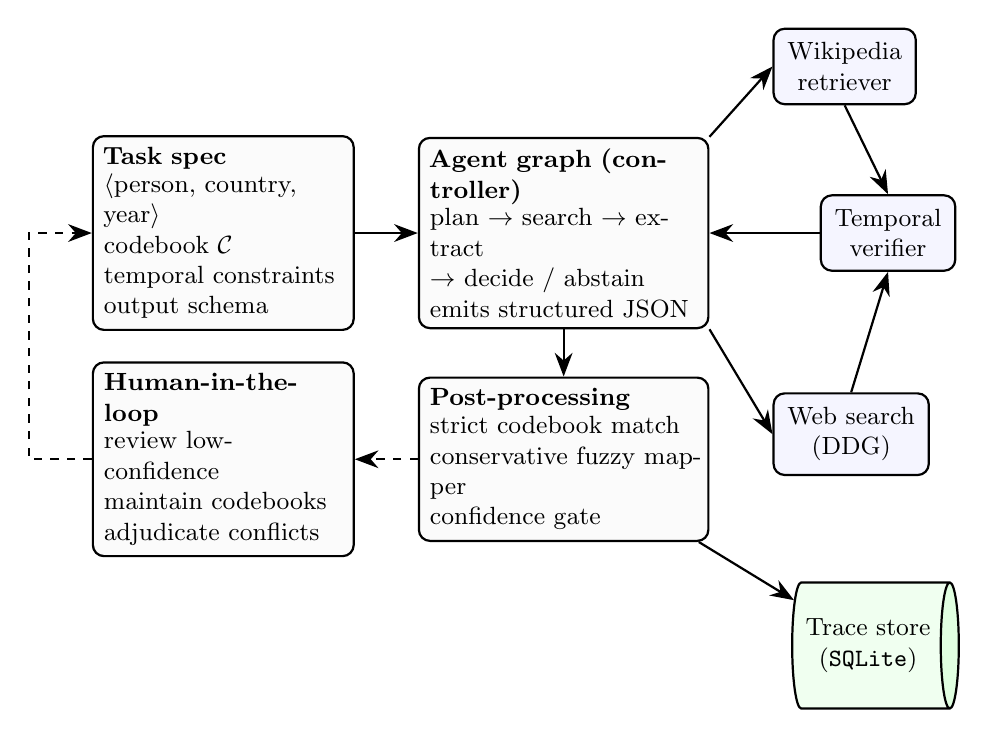
\begin{tikzpicture}[
    font=\small,
    node distance=6mm and 8mm,
    comp/.style={rounded corners, draw=black, thick, fill=gray!3, inner sep=4pt, align=left},
    tool/.style={rounded corners, draw=black, thick, fill=blue!4, inner sep=5pt, align=center},
    store/.style={cylinder, cylinder uses custom fill, cylinder body fill=green!6, cylinder end fill=green!12, draw=black, thick, aspect=0.25, minimum height=18mm, minimum width=16mm, align=center},
    arr/.style={-{Stealth[length=3mm]}, thick},
    loop/.style={-{Stealth[length=3mm]}, thick, dashed},
  ]
    \node[comp, text width=0.25\linewidth] (spec) {
      \textbf{Task spec}\\[-1pt]
      \(\langle\)person, country, year\(\rangle\)\\
      codebook \(\mathcal{C}\)\\
      temporal constraints\\
      output schema
    };

    \node[comp, right=of spec, text width=0.28\linewidth] (graph) {
      \textbf{Agent graph (controller)}\\[-1pt]
      plan \(\rightarrow\) search \(\rightarrow\) extract\\
      \(\rightarrow\) decide / abstain\\
      emits structured JSON
    };

    \node[tool, above right=4mm and 8mm of graph] (wiki) {Wikipedia\\retriever};
    \node[tool, below right=8mm and 8mm of graph] (web) {Web search\\(DDG)};
    \node[tool, right=14mm of graph] (time) {Temporal\\verifier};

    \node[comp, below=of graph, text width=0.28\linewidth] (post) {
      \textbf{Post-processing}\\[-1pt]
      strict codebook match\\
      conservative fuzzy mapper\\
      confidence gate
    };

    \node[store, below right=5mm and 12mm of post] (db) {Trace store\\(\texttt{SQLite})};

    \node[comp, left=of post, text width=0.25\linewidth] (human) {
      \textbf{Human-in-the-loop}\\[-1pt]
      review low-confidence\\
      maintain codebooks\\
      adjudicate conflicts
    };

    \draw[arr] (spec) -- (graph);
    \draw[arr] (graph) -- (post);
    \draw[arr] (post) -- (db);

    \draw[arr] (graph.north east) -- (wiki.west);
    \draw[arr] (graph.south east) -- (web.west);
    \draw[arr] (wiki.south) -- (time.north);
    \draw[arr] (web.north) -- (time.south);
    \draw[arr] (time.west) -- ([xshift=0mm]graph.east);

    \draw[loop] (post.west) -- (human.east);
    % Route this feedback loop outside the "Task spec" box (avoid striking through text).
    \draw[loop] (human.west) -| ([xshift=-8mm]spec.west) -- (spec.west);
  \end{tikzpicture}%
  \caption{Design visualization: a governed agent graph with temporal verification, conservative normalization, abstention, and an auditable trace store.}
  \label{fig:asa-design}
\end{figure}

\subsection{Temporal governance to prevent leakage}

The agent treats time as part of the measurement protocol. Each run is parameterized by an ``as-of'' rule: sources should be published before a cut date (e.g., \(t_i+1\) year) or within a target window around \(t_i\).
When feasible, the system extracts publication dates from retrieved pages and enforces the constraint strictly; otherwise it falls back to best-effort warnings and abstention rather than silently using potentially post-period material.
This guards against a common dataset-construction failure mode: coding pre-period attributes with post-period knowledge.

Temporal controls are crucial because many online sources are retrospective and continuously updated: Wikipedia leads, later biographies, and obituaries often summarize whole careers, including events after \(t_i\). If such post-\(t_i\) material is used to code a pre-period attribute, the measurement can incorporate information that is itself downstream of later outcomes (e.g., a party switch or coalition realignment that occurs after \(t_i\)), creating look-ahead/data leakage and a close analogue of post-treatment conditioning. This can both inflate apparent coding accuracy (by using information unavailable at the time) and bias downstream relationships by contaminating ``baseline'' covariates with post-period events \citep{montgomery2018conditioning,kaufman2012leakage}.

\subsection{Provenance preservation and storage}

All tool interactions and intermediate artifacts are persisted (including URLs and timestamps) to enable:
(i) verification of any individual label by following its citations, (ii) replication of aggregate statistics given the same trace store, and (iii) retrospective audits when codebooks change or new sources appear.
The storage design also supports alternative downstream rules (e.g., only keep labels supported by government sources).

\section{Data and gold standard\label{sec:data}}

We validate ASA on party affiliation, a verifiable elite attribute that is frequently missing in large political-elite panels yet can often be corroborated from public records (party rosters, parliamentary biographies), reputable encyclopedic sources, and contemporaneous news coverage.
The unit of analysis is a leader--record indexed by \(\langle\)person, country, year\(\rangle\).

\subsection{Elite records and country-year codebooks}

For each country-year, domain experts provide a \emph{closed codebook} of admissible party labels.
The codebook enforces cross-national comparability by preventing open-ended label generation, while allowing country-specific party systems to be represented without forcing artificial cross-country harmonization.
When party naming conventions evolve (coalitions, mergers, rebrands), codebooks can be updated and prior labels can be re-audited using the archived traces.

\subsection{Expert labels and evaluation set}

The evaluation set is the subset of leader--records with expert-provided party labels.
We score ASA predictions against expert labels \emph{only} when the agent emits a high-confidence label that can be mapped to the country-year codebook.
Low-confidence outputs are withheld by design (abstention), trading coverage for precision.

\subsection{Outcome definition and temporal target}

The target label is the leader's party affiliation for observation year \(t_i\).
Because elites may switch parties within a year and sources are often retrospective, ASA applies an explicit ``as-of'' rule for admissible evidence.
The precise temporal cut and adjudication rules for within-year switches should be stated alongside the task configuration (Appendix~\ref{sec:appendix-task}).

\section{Validation: party affiliation labeling\label{sec:validation}}

\subsection{Experimental design}

Each record triggers a short, budgeted retrieval episode. The agent is instructed to prioritize verifiable sources, provide citations in its one-sentence justification, and abstain (low confidence) when evidence is weak or conflicting.
Temporal governance is applied as described in Section~\ref{sec:method}: where publication dates can be recovered, post-period sources are excluded; otherwise the agent warns and abstains rather than silently relying on potentially post-period material.

\subsection{Baselines and ablations}

We report performance against a simple baseline that predicts, within each country, the modal party label in the expert-coded evaluation subset.
This captures how much performance comes from exploiting skewed label distributions.
In addition, a standard submission-ready validation should include: (i) an open-world ``search-enabled chat'' baseline without closed codebooks, (ii) a no-temporal-governance ablation, (iii) a no-abstention ablation (forced prediction), and (iv) a strict-match-only ablation (no relaxed mapper).
We provide protocol details for these comparisons in Appendix~\ref{sec:appendix-robustness}.

\subsection{Metrics}

We report (i) accuracy conditional on non-abstention (high confidence), (ii) coverage (the share of records receiving a high-confidence label), and (iii) coverage gain relative to expert-only availability.
Because the unit of analysis is nested within countries, uncertainty should be summarized with country-clustered or country-resampled intervals in a submission-ready version of the paper.

\subsection{Results}

Using the subset of leader--records with expert codings, ASA attains an overall high-confidence accuracy of \LLMOverallAccHighpolparty{} across \LLMNumCountriespolparty{} countries (\(N=\) \LLMNumInstancespolparty{}), while expanding coverage by \LLMNumPredictionsGainedPercentpolparty{}\% (\LLMNumPredictionsGainedpolparty{} records) through conservative augmentation.
Low-confidence outputs are withheld by design, trading recall for precision; the mean share withheld is \LLMMeanLowConfpolparty{}.
Table~\ref{tab:validation-summary} summarizes the key quantities.

\begin{table}[htb]
\centering
\caption{Validation summary for party-affiliation labeling (high-confidence predictions scored against expert labels).}
\label{tab:validation-summary}
\small
\begin{tabularx}{\linewidth}{@{}lX@{}}
\toprule
\textbf{Quantity} & \textbf{Value} \\
\midrule
Countries & \LLMNumCountriespolparty{} \\
Matched leader--records (expert overlap) & \LLMNumInstancespolparty{} \\
Distinct party labels (closed codebooks) & \LLMNumClassespolparty{} \\
High-confidence accuracy (non-abstained) & \LLMOverallAccHighpolparty{} \\
Overall accuracy (all predictions) & \LLMOverallAccAllpolparty{} \\
Mean share withheld (low confidence) & \LLMMeanLowConfpolparty{} \\
Mean country-majority baseline accuracy & \LLMMeanBaselineByCountrypolparty{} \\
Mean uplift over baseline (high confidence) & \LLMMeanDeltaByCountrypolparty{} \\
Coverage gained (new labels) & \LLMNumPredictionsGainedPercentpolparty{}\% (\LLMNumPredictionsGainedpolparty{} records) \\
Accuracy for small/minority parties & \LLMMeanAccSmallGroupspolparty{} \\
Accuracy for large/plurality parties & \LLMMeanAccLargeGroupspolparty{} \\
\bottomrule
\end{tabularx}
\end{table}

\begin{figure}[htb]
  \centering
  \includegraphics[width=0.92\linewidth]{AgentHist.pdf}
  \caption{Agent performance in predicting party across countries with sufficient expert overlap. High-confidence predictions are evaluated against expert labels.}
  \label{fig:agent-performance}
\end{figure}

\begin{figure}[htb]
  \centering
  \includegraphics[width=0.60\linewidth]{AgentOverTime.pdf}
  \includegraphics[width=0.37\linewidth]{AgentRegionBox.pdf}
  \caption{Performance heterogeneity by time (left) and region (right).}
  \label{fig:agent-heterogeneity}
\end{figure}

% Required packages for the tables:
% \usepackage{booktabs}
% \usepackage{array}
% \usepackage{ragged2e}
% \usepackage{tabularx}
% \usepackage[table]{xcolor}
% \usepackage{hyperref}
% \usepackage{threeparttable}
%
% Recommended customizations (preamble):
% \definecolor{RowShade}{gray}{0.96}
% \newcolumntype{P}[1]{>{\RaggedRight\arraybackslash}p{#1}}
% \newcolumntype{C}[1]{>{\Centering\arraybackslash}p{#1}}
% \newcolumntype{Y}{>{\RaggedRight\arraybackslash}X}

\begin{table}[htbp]
\centering
\begingroup\setlength{\tabcolsep}{5pt}\renewcommand{\arraystretch}{1.18}
\begin{threeparttable}
\caption{Sample agent traces. Text content truncated for readability (and may contain typograical errors as present in native source). Links are clickable. Full traces contain many more sources.}
\label{tab:sample_compact}
\scriptsize
\begin{tabularx}{\linewidth}{@{}P{2.8cm}Y@{}}
\toprule
\textbf{Field} & \textbf{Content} \\
\midrule\rowcolor{RowShade}\multicolumn{2}{@{}l}{\textbf{Entry 1:} \textbf{Syleiman Abusaidovich Kerimov} — Russian Federation (1999)} \\
\addlinespace[0.25em]
\textbf{Country} & Russian Federation \\
\textbf{Year} & 1999 \\
\textbf{Person} & Syleiman Abusaidovich Kerimov \\
\textbf{Wikipedia} & Page: Ashot Egiazaryan Summary: Ashot Gevorkovich Egiazaryan (Russian: Ашот Геворкович Егиазарян; Armenian: Աշոտ Գեւորգովիչ Էկիազարյան; born... \\
\textbf{Search 1} & In the spring of 1998, Yeltsin dismissed Chernomyrdin as head of government and in1999Yeltsin's administration backed a newly formedparty,Un... \\
\textbf{URL 1} & \href{https://en.wikipedia.org/wiki/Our_Home_–_Russia https://en.wikipedia.org/wiki/Suleyman_Kerimov}{\footnotesize https://en.wikipedia.org/...} \\
\textbf{Search 2} & OURHOMEISRUSSIAPARTYOurHomeIsRussia(Nash Dom—Rossiya, or NDR) was a sociopolitical movement and a rulingpartyfrom 1996 to 1998. Source for i... \\
\textbf{URL 2} & \href{https://www.encyclopedia.com/history/encyclopedias-almanacs-transcripts-and-maps/our-home-russia-party https://tadviser.com/index.php/Person:Suleyman_Abusaidovich_Kerimov}{\footnotesize https://www.encyclopedia.com/...} \\
\addlinespace[0.35em]\cmidrule(lr){1-2}\addlinespace[0.15em]
\rowcolor{RowShade}\multicolumn{2}{@{}l}{\textbf{Entry 2:} \textbf{Jasminka Stanojevic} — Serbia (2018)} \\
\addlinespace[0.25em]
\textbf{Country} & Serbia \\
\textbf{Year} & 2018 \\
\textbf{Person} & Jasminka Stanojevic \\
\textbf{Wikipedia} & Page: Supreme Court (Serbia) Summary: The Supreme Court (Serbian: Врховни суд, romanized: Vrhovni sud) is the court of last resort in Serbia... \\
\textbf{Search 1} & This article lists political parties inSerbia, including parties that existed in the Kingdom ofSerbiabetween the early 1860s and 1918. A kol... \\
\textbf{URL 1} & \href{https://en.wikipedia.org/wiki/List_of_political_parties_in_Serbia https://www.kurir.rs/vesti/politika/2891361/22-godina-od-egzodusa-srba-u-oluji-ocajna-jasminka-stanojevic-deca-su-se-godinama-nadala-da-je-otac-ziv}{\footnotesize https://en.wikipedia.org/...} \\
\textbf{Search 2} & Imali su dve i četiri godine kad smo izbegli iz Knina. Kad bi neko pokucao na vrata, vikali bi: „Tata, tata". Tri godine nakon progona sazna... \\
\textbf{URL 2} & \href{https://www.kurir.rs/vesti/politika/2891361/22-godina-od-egzodusa-srba-u-oluji-ocajna-jasminka-stanojevic-deca-su-se-godinama-nadala-da-je-otac-ziv https://www.facebook.com/public/Jasminka-Stanojevic/}{\footnotesize https://www.kurir.rs/...} \\
\addlinespace[0.35em]\cmidrule(lr){1-2}\addlinespace[0.15em]
\rowcolor{RowShade}\multicolumn{2}{@{}l}{\textbf{Entry 3:} \textbf{Mihai STROE} — Romania (2011)} \\
\addlinespace[0.25em]
\textbf{Country} & Romania \\
\textbf{Year} & 2011 \\
\textbf{Person} & Mihai STROE \\
\textbf{Wikipedia} & Page: Adrian Stroe Summary: Adrian Stroe (born 24 October 1959), known as The Taxi Driver of Death, is a Romanian serial killer responsible ... \\
\textbf{Search 1} & Născut în Bucureşti şi cu origini în comuna argeşeană Morăreşti, fost medaliat cu aur la olimpiada internaţională de informatică,MihaiStroe(... \\
\textbf{URL 1} & \href{https://adevarul.ro/stiri-locale/pitesti/povestea-fascinanta-a-romanului-care-a-ajuns-1720222.html https://www.cdep.ro/pls/parlam/structura2015.mp?idm=286\&cam=2\&leg=2008\&pag=0 https://www.youtube.com/mihaistroetv}{\footnotesize https://adevarul.ro/...} \\
\textbf{Search 2} & MihaiSTROEParliamentary activity in legislature 2008-2012 DEPUTY Constituency no.38 TULCEA, uninominal college no.2 Membru al PDL, deputatul... \\
\textbf{URL 2} & \href{https://www.cdep.ro/pls/parlam/structura2015.mp?idm=286\&cam=2\&leg=2008\&idl=2 https://adevarul.ro/stiri-locale/tulcea/deputatul-democrat-liberal-mihai-stroe-nu-cred-1118196.html https://www.instagram.com/stroemihai/}{\footnotesize https://www.cdep.ro/...} \\
\addlinespace[0.35em]\cmidrule(lr){1-2}\addlinespace[0.15em]
\rowcolor{RowShade}\multicolumn{2}{@{}l}{\textbf{Entry 4:} \textbf{Matsie Angelina Motshekga} — South Africa (2018)} \\
\addlinespace[0.25em]
\textbf{Country} & South Africa \\
\textbf{Year} & 2018 \\
\textbf{Person} & Matsie Angelina Motshekga \\
\textbf{Wikipedia} & Page: Angie Motshekga Summary: Matsie Angelina "Angie" Motshekga (born 19 June 1955) is a South African politician and educator who is curre... \\
\textbf{Search 1} & MatsieAngelina"Angie"Motshekga(born 19 June 1955) is a SouthAfricanpolitician and educator who is currently serving as the Minister of Defen... \\
\textbf{URL 1} & \href{https://en.wikipedia.org/wiki/Angie_Motshekga}{\footnotesize https://en.wikipedia.org/wiki/Angie\_Motshekga} \\
\textbf{Search 2} & Motshekgawas elected thenationalpresident of theAfricanNationalCongressWomen's League (ANCWL) in 2008, defeating the League's secretary-gene... \\
\textbf{URL 2} & \href{https://www.sahistory.org.za/people/matsie-angelina-motshekga-angie-motshekga}{\footnotesize https://www.sahistory.org.za/people/matsie-angelina-motshekga-angie-motshekga} \\

\bottomrule
\end{tabularx}
\begin{tablenotes}
\footnotesize
\item 
\end{tablenotes}
\end{threeparttable}
\endgroup
\end{table}


\subsection{Auditability and trace-based verification}

The core advantage of ASA over unconstrained chat workflows is that each accepted label can be audited by inspecting its citations and full trace.
The trace store preserves the queries, retrieved snippets, URLs, and timestamps used during coding, enabling replication and retrospective re-analysis when sources change or when users adopt stricter inclusion rules (e.g., accept only government sources).
Table~\ref{tab:sample_compact} illustrates the resulting evidence-first trace style: multiple sources are retrieved and recorded alongside links, allowing a reader to verify what evidence the label relied on under the declared temporal rule.

\begin{figure}[htb]
\centering
\fbox{\begin{minipage}{0.95\linewidth}
\small
\textbf{Worked example: why ``as-of'' governance matters.}
Consider a record with observation year \(t_i\) and a label intended to reflect the pre-period state (e.g., party affiliation at \(t_i\)).
A naive workflow that reads a current biography or Wikipedia lead may inadvertently use retrospective summaries that incorporate events after \(t_i\), creating look-ahead/data leakage \citep{kaufman2012leakage} and a close analogue of post-treatment conditioning \citep{montgomery2018conditioning}.
ASA instead treats time as part of the measurement protocol: it constrains retrieval to sources published before a cut date (or within a target window), and it abstains when the available evidence cannot be shown to be pre-period.
Table~\ref{tab:sample_compact} illustrates the resulting trace style: multiple sources are retrieved and recorded alongside URLs, allowing a reader to verify what evidence the label relied on under the declared temporal rule.
\end{minipage}}
\caption{A compact intuition for temporal governance and trace-based verification.}
\label{fig:worked-example}
\end{figure}

\section{Discussion: design tradeoffs and practical guidance}

\paragraph{Cost and scaling.}
The methodology is built for high throughput: each record triggers a short, budgeted tool-usage episode and yields a structured output that can be scored, filtered, and aggregated without manual parsing.
Using smaller instruction-tuned models for orchestration, caching retrieval outputs, and routing only uncertain cases to humans yields substantial cost savings relative to fully manual coding or repeated interactive browsing.

\paragraph{What this approach does (and does not) guarantee.}
Provenance capture makes the \emph{evidence} for each label inspectable, but it does not magically eliminate ambiguity in the world.
The point of abstention is to keep ambiguity from silently becoming noise.
Similarly, temporal governance reduces leakage risk, but cannot fully recover historical truth when the web record is sparse.
In practice, auditability means a downstream user can inspect a label by following its recorded citations and can re-apply alternative inclusion rules (e.g., require government sources only) using the archived trace, consistent with calls for reproducible computational work \citep{peng2011reproducible,stodden2013toward}.
Key failure modes include (i) sources without reliable publication dates, (ii) sparse historical web records for earlier years, and (iii) entities with name ambiguity across languages; ASA responds by warning, tightening evidence requirements, and abstaining rather than imputing.

\paragraph{When to use ASA.}
ASA is best suited to \emph{verifiable attributes} with authoritative sources (party membership, office holding, election outcomes) and stable codebooks.
For sensitive or non-verifiable attributes (e.g., ethnicity without self-identification), we recommend stricter abstention and explicit ethical review.

\section{Transparency, reproducibility, and data availability\label{sec:transparency}}

ASA produces two primary research artifacts: (i) a structured dataset of labels (including abstentions and confidence flags), and (ii) an auditable trace store that documents the evidence environment that produced each label.
To support replication, a submission-ready package should (a) freeze the trace store used for reported results, (b) include scripts that reproduce all tables and figures from the frozen store, and (c) document the task specification (codebooks, temporal rules, output schema).

Because the underlying elite panel and full trace store may be subject to access constraints, we recommend a controlled-access transparency strategy: release the \texttt{asa} software, schema definitions, and de-identified example traces immediately; and provide reviewers (and later readers) with an access pathway for full traces and expert codebooks consistent with ethical and legal constraints.

\section{Limitations and ethical/legal considerations\label{sec:limitations}}

\paragraph{Dynamic sources and dating.}
Web sources evolve (link rot, edits, retroactive updates), and many pages lack reliable publication dates.
Temporal governance reduces leakage risk but cannot guarantee that all evidence is contemporaneous; abstention is therefore a feature, not a bug.

\paragraph{Coverage and representation bias.}
Evidence quality varies systematically by language, region, and historical period, and across types of elites.
These differences can create uneven missingness and error that must be documented and, where possible, modeled downstream.

\paragraph{Terms of service and privacy.}
Web retrieval should respect site terms, robots policies, and privacy considerations.
Trace storage policies should minimize unnecessary retention of personal data while preserving enough evidence for audit (e.g., store URLs and short snippets rather than bulk page content when feasible).

\section{Conclusion}

For political-elite research, the central question is not whether LLMs can answer factual questions, but whether they can be integrated into a \emph{measurement protocol} that is auditable, comparable, temporally well-defined, and cost-effective at scale.
The verifiable search agent methodology operationalizes these requirements through closed codebooks, evidence-first outputs, strict trace preservation, and conservative abstention.
This design turns retrieval-augmented agents into replicable instruments for dataset construction rather than opaque assistants.

\section*{Acknowledgments}
\noindent \textit{[To be completed prior to submission.]}

\section*{Funding}
\noindent \textit{[To be completed prior to submission.]}

\section*{Competing interests}
\noindent \textit{[To be completed prior to submission.]}

\section*{Author contributions}
\noindent \textit{[To be completed prior to submission.]}

\appendix
\section{Task specification for party affiliation\label{sec:appendix-task}}

This appendix documents the task-level specification used in the party-affiliation validation: the required output schema, the country-closed normalization rules, the confidence gate (abstention policy), and a representative prompt template.

\subsection{Structured output schema}

For each record \(\langle\)person, country, year\(\rangle\) the agent returns a single JSON object.
In the party-affiliation task, we require (at minimum) the following fields:
\begin{itemize}[leftmargin=*, itemsep=2pt]
\item \texttt{pol\_party}: a single party label chosen from the country-year codebook (exact string match).
\item \texttt{justification}: one sentence that cites the evidence supporting the label.
\item \texttt{confidence}: a categorical confidence flag (High, Medium, Low).
\end{itemize}
The trace store separately records the evidence environment (queries, snippets, URLs, timestamps) used to generate the output.

\subsection{Country-closed matching and normalization}

To guard cross-national comparability and reduce typographic drift, we apply a two-stage, codebook-guided normalization to the model's raw label string:
\begin{enumerate}[leftmargin=*, itemsep=2pt]
\item \textbf{Strict closed-set match (country scope).} If the predicted string exactly matches a member of the country-year codebook, it is accepted.
\item \textbf{Conservative fuzzy match.} Otherwise, a relaxed mapper computes a similarity score \(s\) combining (a) Jaro--Winkler similarity on a normalized label, (b) token overlap coverage, and (c) acronym equality.
Let \(m\) denote the runner-up score.
Accept as a match if
\[
s \ge 0.92 \quad \text{or} \quad \bigl(s \ge 0.85 \ \&\  s-m \ge 0.08\bigr).
\]
\end{enumerate}
This mapping process produces a normalized label used for evaluation and aggregation while preserving the original string for audit.
It corrects innocuous variants (pluralization, punctuation, acronyms) without introducing new classes.
In the party-affiliation case study, the relaxed mapper changes \LLMRelaxedChangedPctpolparty{}\% of accepted labels.

\subsection{Confidence gate and abstention policy}

The agent emits a categorical confidence estimate.
Records flagged \texttt{Low} (and, in conservative downstream analyses, \texttt{Medium}) are withheld from automated use, implementing an abstention layer that trades coverage for precision.
Abstention is most common where web evidence is sparse, parties are newly formed, transliterations vary, or publication dates cannot be verified under the ``as-of'' rule.

\subsection{Representative prompt template}

\begingroup
\footnotesize
\begin{verbatim}
TASK OVERVIEW:
You are a search-enabled language model performing
party affiliation inference.
Your goal is to identify the political party of a
specified individual in a specified country and year,
using retrieved evidence. If evidence is weak or
conflicting, you must abstain by returning
confidence = "Low".

TARGET RECORD:
- Name: <PERSON_NAME>
- Country: <COUNTRY>
- Observation year: <YEAR>
- Parties (closed codebook): [<PARTY_1>, <PARTY_2>, ...]

CONSTRAINTS:
1. You MUST choose exactly ONE party from the closed
   codebook for pol_party when confidence is High or
   Medium.
2. You MUST NOT invent a party not in the codebook.
3. The selected party string must exactly match the codebook entry.
4. Write all explanations in English and cite sources.

RESPONSE FORMAT (JSON ONLY):
{
  "justification": "One sentence with citations to retrieved sources.",
  "pol_party": "Exact party label from the codebook",
  "confidence": "High|Medium|Low"
}
\end{verbatim}
\endgroup

\section{Recommended additional validation for submission\label{sec:appendix-robustness}}

To meet common journal expectations for a submission-ready measurement paper, the validation section should include:
\begin{itemize}[leftmargin=*, itemsep=2pt]
\item \textbf{Open-world baseline:} a ``search-enabled chat'' workflow without closed codebooks and without trace enforcement.
\item \textbf{No temporal governance ablation:} remove the ``as-of'' constraint and show the effect on accuracy/coverage (and leakage risk).
\item \textbf{No abstention ablation:} force a label on all records and report the precision--coverage tradeoff.
\item \textbf{Strict-match-only ablation:} remove the relaxed mapper to quantify the role of normalization.
\item \textbf{Uncertainty summaries:} country-clustered or country-resampled intervals for headline metrics.
\end{itemize}

\section{Trace store fields\label{sec:appendix-trace}}

The ASA trace store is designed to make each measurement auditable.
At minimum, it records (a) the record identifier and task configuration (including the codebook and temporal rule), (b) each retrieval action (query strings, tool responses, extracted snippets), and (c) the final structured output with confidence.
This enables retrospective audits (follow the citations), re-filtering (apply stricter evidence rules), and reproducible aggregate statistics from a frozen trace store.


\printbibliography

\end{document}
